% CVPR 2024 Paper Template; see https://github.com/cvpr-org/author-kit

\documentclass[10pt,twocolumn,letterpaper]{article}

\usepackage{cvpr}              
% To produce the CAMERA-READY version
\usepackage{algorithm}
\usepackage{algpseudocode}
\usepackage{appendix}


%
% --- inline annotations
%
\usepackage[dvipsnames]{xcolor}
\newcommand{\red}[1]{{\color{red}#1}}
\newcommand{\todo}[1]{{\color{red}#1}}
\newcommand{\TODO}[1]{\textbf{\color{red}[TODO: #1]}}
% --- disable by uncommenting  
% \renewcommand{\TODO}[1]{}
% \renewcommand{\todo}[1]{#1}



\definecolor{cvprblue}{rgb}{0.21,0.49,0.74}
\usepackage[pagebackref,breaklinks,colorlinks,citecolor=cvprblue]{hyperref}
\usepackage[utf8]{inputenc}

\usepackage{graphicx}
\usepackage{multicol}

\def\paperID{*****} % *** Enter the Paper ID here
\def\confName{CVPR}
\def\confYear{2024}

\title{is-that-A-CART: A Preliminary Framework for Automated Shopping Cart Retrieval in Retail Environments with YOLOv8}

\author{Wentao Jiang\\
University of Rochester\\
500 Joseph C. Wilson Blvd., NY 14627\\
{\tt\small wjiang20@u.rochester.edu}
\and
Alvin Jiang\\
University of Rochester\\
500 Joseph C. Wilson Blvd., NY 14627\\
{\tt\small yjiang54@u.rochester.edu}
\and
Arthur Masiukiewicz\\
University of Rochester\\
500 Joseph C. Wilson Blvd., NY 14627\\
{\tt\small amasiuki@u.rochester.edu}
}


\begin{document}
\maketitle

\begin{abstract}
Upon concluding their shopping experience, patrons exiting markets may leave store-owned shopping carts at various locations within the environment without heeding the potential consequences. For instance, carts scattered around retail environments may lead to traffic blockage, and carts on parking spaces may prevent vehicles from parking there. Currently, retail stores such as Target\raisebox{1pt}{\textregistered}\ and Wegmans\raisebox{1pt}{\textregistered}\ hire human resources to retrieve shopping carts and gather them at a specific location for recycling. However, our goal is to automate this process by incorporating computer vision technologies. For our study, we train and fine-tune the \textbf{YOLOv8} (You Only Look Once, version 8) network, a state-of-the-art computer vision model, to perform bounding box detection. In addition, we propose a framework with machine integration to streamline shopping trolley retrieval.
\end{abstract}

\section{Introduction}
Managing shopping cart locations presents a considerable logistical challenge in modern retail environments. Customers often leave carts scattered throughout the store, parking areas, and store vicinity, resulting in traffic disruptions and inefficient parking space usage. Furthermore, unattended objects in public may raise security concerns for general public safekeeping~\cite{abandoned-cart}, necessitating extraneous attention in the surveillance process. Traditionally, stores like Target and Wegmans employ human labor to streamline this process. However, we would like to propose a framework that automates the retrieval of shopping trolleys involving computer vision and robotics technologies. Toward this end, we aim to train a model and achieve high performance on shopping cart segmentation from images. In addition, we would also like to present a holistic review of the modern landscape of robotics and how machine vision technologies can be involved during shopping trolley retrieval.

The remainder of this paper is organized as follows: Section 2 discusses related works in the field, Section 3 describes the methods employed in our study, Section 4 presents our experimental analysis and results, Section 5 reviews the current landscape of robotics in the context of object retrieval, Section 6 presents a preliminary framework for cart retrieval, and Section 7 discusses these findings in the context of existing literature and potential future approach. 

\section{Related Work}
Melegrito et al.~\cite{abandoned-cart} presented their findings using the YOLOv3 network for detecting abandoned shopping carts in parking areas. This approach achieved both high training and validation accuracy and precision in identification. This study highlighted the YOLO model's potential application in retail management and operational efficiency. Despite the similarity to this article, our study implements shopping trolley detection in various environments, highlighting its uniqueness in its field of study.

Jadhav and Momin~\cite{detection-identifcation} contributed to an identification task of abandoned objects in public through the lens of video surveillance systems. The scholars utilized a dual-background, hybrid model efficient and reliable for stationary object detection. After detection, they extracted object attributes such as height, width, size, color, and time. Their study spearheaded potential future direction for our research to classify whether detected shopping carts have been unattended.

Albeit not directly related to object detection and retrieval, Wagner et al.'s article~\cite{wagner} provided meaningful insights on the implications of in-store shopping cart movements on consumer shopping behavior. Through disguised observational studies, their aggregate data revealed that shopping trolley placement and movement impacted the duration of a consumer's visit, paths taken within the store, and interaction with products.

\section{Methods}

\subsection{Dataset}
We obtained Kornilov's "shopping trolley" dataset~\cite{kornilov-dataset} from Roboflow to train the YOLOv8 network and to test the model's performance.

\subsubsection{Data Volume}
Kornilov's dataset~\cite{kornilov-dataset} comprises a total of 6903 images collected from diverse retail environments to ensure a comprehensive representation of various scenarios involving shopping cart placement. The dataset's split ratio is as follows:

\begin{table}[h]
\centering
\begin{tabular}{lcc}
\hline
\textbf{Dataset Split} & \textbf{Number of Samples} & \textbf{Percentage of Total} \\
\hline
Training Set     & 5,996 & 87\% \\
Validation Set   & 461   & 7\%  \\
Test Set         & 446   & 6\%  \\
\hline
\end{tabular}
\caption{Dataset Split}
\label{tab:dataset_split}
\end{table}

While the train-test-split ratio deviates from the conventional allocations, which have a smaller training ratio, this variance is justifiable given the substantial volume of~\cite{kornilov-dataset}. Larger datasets can effectively support different split ratios without compromising the validation and performance of the models, as proposed by Rácz et al.~\cite{molecules}.

\subsubsection{Data Measurements}

\begin{table}[ht]
\centering
\begin{tabular}{lcccc}
\hline
\textbf{Color Channel} & \textbf{Mean} & \textbf{Stdev} \\ 
\hline
Red & 0.587 & 0.199 \\
Green & 0.558 & 0.203 \\
Blue & 0.534 & 0.206 \\
\hline
\end{tabular}
\caption{RGB Description of the Original Dataset (normalized)}
\end{table}
For comparison, the default \textit{ImageNet} normalization parameters are mean = [0.485, 0.456, 0.406] and std = [0.229, 0.224, 0.225].

Overall, these statistics suggest that Kornilov's dataset~\cite{kornilov-dataset} contains a diverse set of images with no extreme bias towards any particular color. The high standard deviation values of red, green, and blue confirm the presence of diverse image content and/or varying lighting conditions. 

\subsubsection{Data Annotation}
The ground truth values have been pre-labeled by the author of the dataset~\cite{kornilov-dataset}. Specifically, these values are bounding boxes that highlight shopping carts within the images in the dataset. Each bounding box is defined by the centerX, centerY, width, and height that specify the rectangular area covering a shopping cart. 

\subsubsection{Image Augmentation}
The preprocessing pipeline integrates a suite of advanced image enhancement and augmentation methods to adapt and scale for the inclusion of additional techniques as needed. To further enhance the model's ability to generalize across different scenarios, we employ a mix of geometric and photometric transformations to enhance the model’s ability to generalize across varied real-world conditions. Additionally, we have configured our system to save these transformed images, which facilitates a thorough inspection of the preprocessing effects but also aids in fine-tuning the model by providing a diverse array of training examples.
% TODO: What transform did you guys use? Add to itemize if there's more and Please change the resized to a \(640 \times 640\) resolution according to the model pixels u trained.
\begin{itemize}
    \item \textbf{Resizing and Cropping}: Images were resized to \(640 \times 640\) pixels to ensure consistency in input dimensions across the dataset, and to fit within the standard used for YOLOv8. Post resizing, a dynamic cropping strategy was implemented for test set, where images were scaled between 80\% and 100\% of their initial size, maintaining an aspect ratio from \(3/4\) to \(4/3\). This helps the model in detecting shopping carts from varying distances and partial views.
    \item \textbf{Random Vertical Flip}: Each image in the test set had a 50\% probability of undergoing a vertical flip. This transformation enhances the dataset's variance by simulating different possible orientations of shopping carts, essential for robust detection.
    \item \textbf{Color Jittering}: To further augment the dataset and account for varying lighting conditions that might affect the appearance of shopping carts, we applied color jittering. This transformation randomly adjusts the brightness, contrast, saturation, and hue of the images, thereby simulating different times of day and lighting conditions found in typical retail environments.
\end{itemize}

\subsubsection{Data Preparation}
In processing the annotations, we prioritized the largest object in each image as the primary label, based on its spatial dimensions. This approach was adopted to enhance accuracy and reflect real-world scenarios where the most prominent object is often of the highest relevance.

Figures \ref{fig:preprocessing1} and \ref{fig:preprocessing2} show a sample image from our dataset after applying the preprocessing steps outlined above.

\begin{figure}[ht]
    \centering
    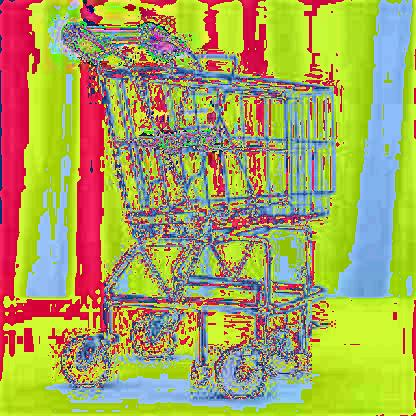
\includegraphics[width=0.3\textwidth]{images/sp--13-_jpg.rf.95ce9b940a8c4ff08ff4b258cb562072.jpg}
    \caption{Example of a preprocessed image showing resized and cropped dimensions in the Train Set.}
    \label{fig:preprocessing1}
\end{figure}

\begin{figure}[ht]
    \centering
    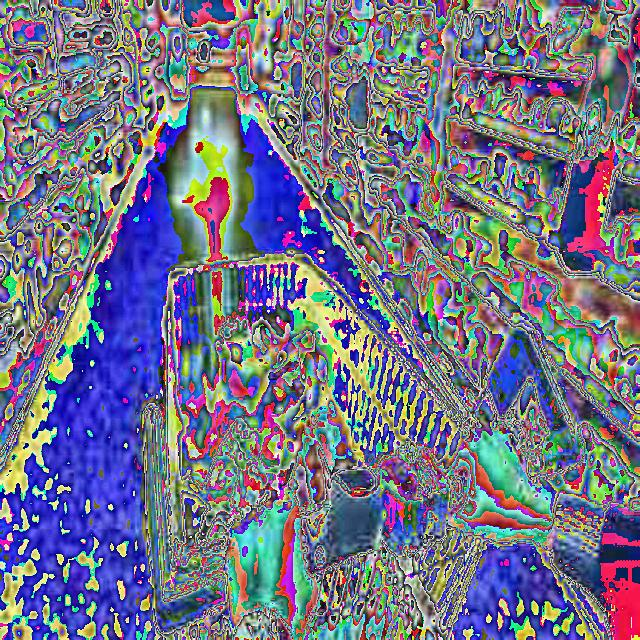
\includegraphics[width=0.3\textwidth]{images/sp--228-_jpg.rf.7d3048d4b2fdd61f2dec2aacf2d05809.jpg}
    \caption{Example of a preprocessed image showing resized and cropped dimensions in the Test Set.}
    \label{fig:preprocessing2}
\end{figure}

\vspace{15pt}

\subsection{YOLOv8 Model}
\subsubsection{Model Analysis}
The transfer-learning type YOLOv8 model employs several advanced techniques common in convolutional neural networks (CNNs), specifically tailored for object detection. This model is ideal for real-time applications due to its ability to process images rapidly while maintaining high accuracy. Below is a detailed analysis of its components and how they contribute to the task of shopping cart detection, referencing the official \textit{PyTorch} documentation~\cite{pytorch}:

\begin{itemize}
    \item \textbf{Convolutional Layers (Conv2d)}: These layers are the primary feature extractors in the network. By applying varying numbers of filters, they capture both low-level features such as edges and textures, and high-level features like the shapes of shopping carts. The varying kernel sizes and strides enable the model to detect carts at different scales and orientations.

    \item \textbf{Batch Normalization (BatchNorm2d)}: This technique is used to stabilize and speed up the deep network training. It normalizes the activation of a previous layer at each batch, maintaining the mean output close to 0 and the output standard deviation close to 1, which improves gradient flow, allows higher learning rates and reduces the sensitivity to initial weights. Normalizing layer outputs ensures that the network behaves consistently across different training batches, which is vital when adapting the model to diverse lighting and background conditions in parking lots or store entries

    \item \textbf{SiLU Activation}: Sigmoid Linear Unit, defined as $f(x) = x \cdot \sigma(x)$. It offers a balance between ReLU and sigmoid functions. The SiLU activation function helps the model make more effective use of the information it processes by allowing gradients to flow better during backpropagation. This property is particularly beneficial in complex scenes where shopping carts might be partially obscured or overlap with other objects.

    \item \textbf{Skip Connections and Bottlenecks}
    \begin{itemize}
        \item \textbf{Skip Connections} ensure that the model retains important information from early in the network, aiding in the accurate reconstruction of the detected objects in the final output layers. This feature helps preserve the detailed features of carts across the network, i.e., mitigate the vanishing gradient problem.
        \item \textbf{Bottleneck Layers} effectively reduce the computational burden by minimizing the number of parameters, allowing the model to operate efficiently without sacrificing performance—key for deploying the model in systems with real-time constraints.
    \end{itemize}

    \item \textbf{SPPF (Spatial Pyramid Pooling - Fast)}: An adaptation of the Spatial Pyramid Pooling layer. This layer ensures that the network can handle input images of varying sizes, making it robust to different camera setups and operational fields without requiring reconfiguration of the network for each new camera or viewpoint.

    \item \textbf{Upsampling and Concatenation}
    \begin{itemize}
        \item \textbf{Upsampling} is used to increase the resolution of the feature maps from deep in the network, which enhances the model's ability to locate and delineate shopping carts precisely within the image.
        \item \textbf{Concatenation} merges feature maps from different layers, allowing the model to use both detailed texture information and higher-level shape information to improve detection accuracy.
    \end{itemize}

    \item \textbf{ModuleList}: This component normally works as a PyTorch container. It provides the architectural flexibility needed to customize the model for specific tasks like shopping cart detection and allows for the easy addition or modification of layers as new challenges or data types are encountered in different retail environments.

\end{itemize}

\subsubsection{Task-specific Deployment} 
We decided to deploy pre-trained YOLOv8 models of the "nano" variety, meaning models containing roughly ~3M parameters. We examined two versions of YOLOv8n, one which was trained initially trained on the COCO (Common Objects in Context) and one on the OpenImagesV7 dataset. In addition, we examined the performance of training YOLOv8n from scratch on our dataset without prior pre-training. Aside from the obvious difference between training from scratch and training a model with previously pre-trained weights, it is important to discuss both datasets used to distinguish between possible future performance differences between both pre-training .

The COCO 2017 dataset is a large-scale object detection, segmentation, and captioning dataset, with over 140k images with 5 objects per image. The bounding boxes are labeled via 91 different classes derived from complex everyday scenes, with shopping trolley, or any version of 'cart' not present as a label~\cite{coco}. The annotation for COCO was completed manually via Amazon Mechanical Turk, where human workers manually segmented each object instance, and multiple annotators were instructed to confirm the presence of categories and accuracy of instance segmentation~\cite{microsoft_coco}.
    
The OpenImagsV7 (OIV7) is an even larger scale dataset; composed of 9 million images, with an average of 8.3 objects per image. The dataset contains bounding boxes dispersed among 600 various categories, with 'cart' being present as one of the 600 categories~\cite{openimagesv7} It is important to note that we are focusing on the detection of shopping carts (trolleys) specifically. However, we expect some shopping carts to be present in the pre-training set with the cart label due to the diverse meaning of the word, and hypothesize that some presence of shopping carts during pre-training will improve this final models' performance. OIV7 was annotated using manual annotators and extreme clicking, where annotators define the most extreme points of an object to form a bounding box - potentially resulting in less precise annotations than COCO - however the larger magnitude of the dataset will most likely outweigh this loss in precision~\cite{openimagesv4}.

Leveraging pre-trained weights allows us to benefit from the model's pre-established feature extraction abilities, significantly reducing the need for extensive training from scratch and ensuring faster convergence. This is due to potentially more effective starting weights for our task, present after pre-training. When pre-training, weights are optimized for specific features seen in the datasets used for pre-training. This is an optimized starting point for future feature activations, as they are more relevant from the beginning when training, resulting in faster convergence. When training from scratch weights are randomly initialized, usually from a specified distribution, thus more adjustments to weights are required during back propagation to generalize to the desired dataset. As such, pre-trained models usually generalize better after final training~\cite{why_does}.

We trained the YOLOv8 model with the training set of Kornilov's dataset~\cite{kornilov-dataset} and the following parameters:

\begin{itemize}
    \item{\textbf{Batch Size:}}
    The training was conducted with a batch size of 25 and a total of 5996 images in the training set. This batch size ensures that enough data is processed per update to capture significant patterns without straining the computational resources.
    \item{\textbf{Epochs:}}
    We trained the model for 100 epochs, allowing multiple iterations over the entire dataset to refine the model weights. This number of epochs was selected to balance between achieving thorough learning and preventing overfitting. This approach ensures the model performs well in real-world conditions.
\end{itemize}

All training processes were executed on a system equipped with NVIDIA{\textregistered} GeForce{\textregistered} RTX 3090 Ti Graphical Processing Unit, featuring 24 GB of VRAM.

\section{Experiment}
To examine the performance of our various model checkpoints, we used the 446 image test set found in Kornilov's dataset~\cite{kornilov-dataset}. To assess the models' performance during testing, we needed to find a method appropriate to examine how well the inferred class instances matched the ground truth of each image in the dataset, when there multiple ground truth bounding boxes, and thus multiple model predictions throughout the image. 

We followed the guidance given by Di Yuan et al.: in their Accurate Bounding-box Regression with Distance-IOU Loss for Visual Tracking paper~\cite{accurate}. We created a function the operates by calculating the Intersection over Union (IoU) for each predicted box against each ground truth bounding box in a given image. If the IoU for a ground truth box exceeds a threshold of 0.5 (majority crossover), the prediction is considered a true positive. Predictions not matching any ground labels were counted as False Positives, and ground truth labels without any matching predictions were counted as False Negatives. If multiple predictions meet the threshold, the prediction with the highest IoU that exceeded the threshold was selected as the match.

The following equations detail how IoU was calculated in our process. First, corners of each bounding box are calculated, by converting the width, height, and center coordinates, to the top-left and bottom-right corners of each box.

\[
x_{\text{min}} = x - \frac{w}{2}, \quad y_{\text{min}} = y - \frac{h}{2}
\]
\[
x_{\text{max}} = x + \frac{w}{2}, \quad y_{\text{max}} = y + \frac{h}{2}
\]

Then, the intersection coordinates are calculated, otherwise known as the coordinates of the overlapping area between two boxes.
\[
x_{\text{left}} = \max(x_{1_{\text{min}}}, x_{2_{\text{min}}}), \quad y_{\text{top}} = \max(y_{1_{\text{min}}}, y_{2_{\text{min}}})
\]
\[
x_{\text{right}} = \min(x_{1_{\text{max}}}, x_{2_{\text{max}}}), \quad y_{\text{bottom}} = \min(y_{1_{\text{max}}}, y_{2_{\text{max}}})
\]

Area of Intersection is calculated by computing the area of the intersecting rectangle found above.

\[
\text{Area of Intersection} = (x_{\text{right}} - x_{\text{left}}) \times (y_{\text{bottom}} - y_{\text{top}})
\]

The area of the two intersecting boxes are then calculated when there is an intersection.

\[
\text{Area of Box}_1 = (x_{1_{\text{max}}} - x_{1_{\text{min}}}) \times (y_{1_{\text{max}}} - y_{1_{\text{min}}})
\]
\[
\text{Area of Box}_2 = (x_{2_{\text{max}}} - x_{2_{\text{min}}}) \times (y_{2_{\text{max}}} - y_{2_{\text{min}}})
\]

Area of Union is calculated by adding the area of both boxes and subtracting the area of intersection from the sum.

\[
\text{Area of Union} = \text{Area of Box}_1 + \text{Area of Box}_2 - \text{Area of Intersection}
\]

Finally, the IoU is calculated by dividing the area of intersection by the area of union.

\[
\text{IoU} = \frac{\text{Area of Intersection}}{\text{Area of Union}}
\]

The final output displayed in Figure 3, is the average overall IoU for the dataset for each model, where all IoUs are summed and divided by the amount of images in the dataset.

\[
\text{Overall IoU} = \frac{1}{N} \sum_{i=1}^{N} \text{IoU}_i
\]

\begin{figure}[H]
    \centering
    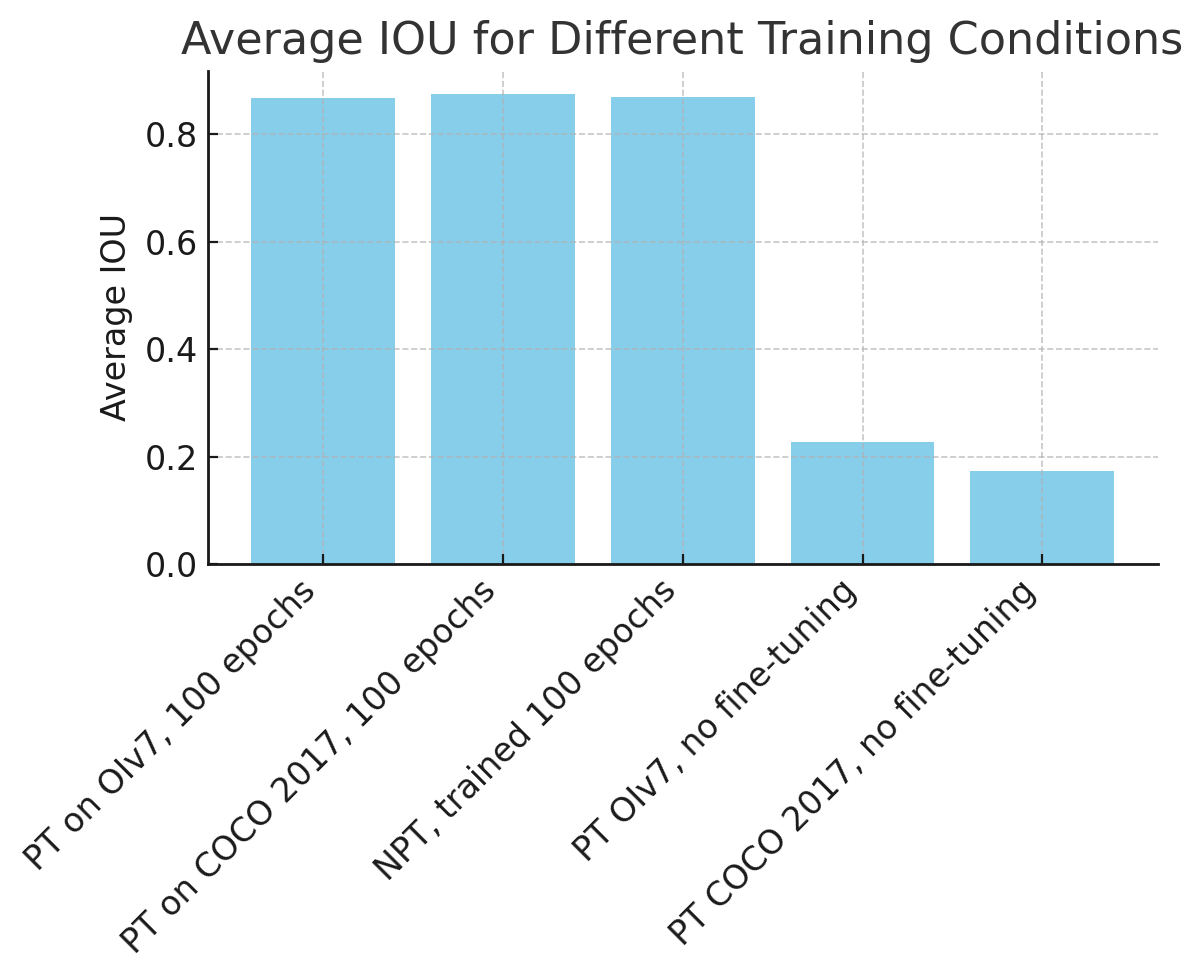
\includegraphics[width=0.8\linewidth]{iou.png}
    \caption{Average IoU across different training conditions}
    \label{fig:iou}
\end{figure}

\begin{figure}[H]
    \centering
    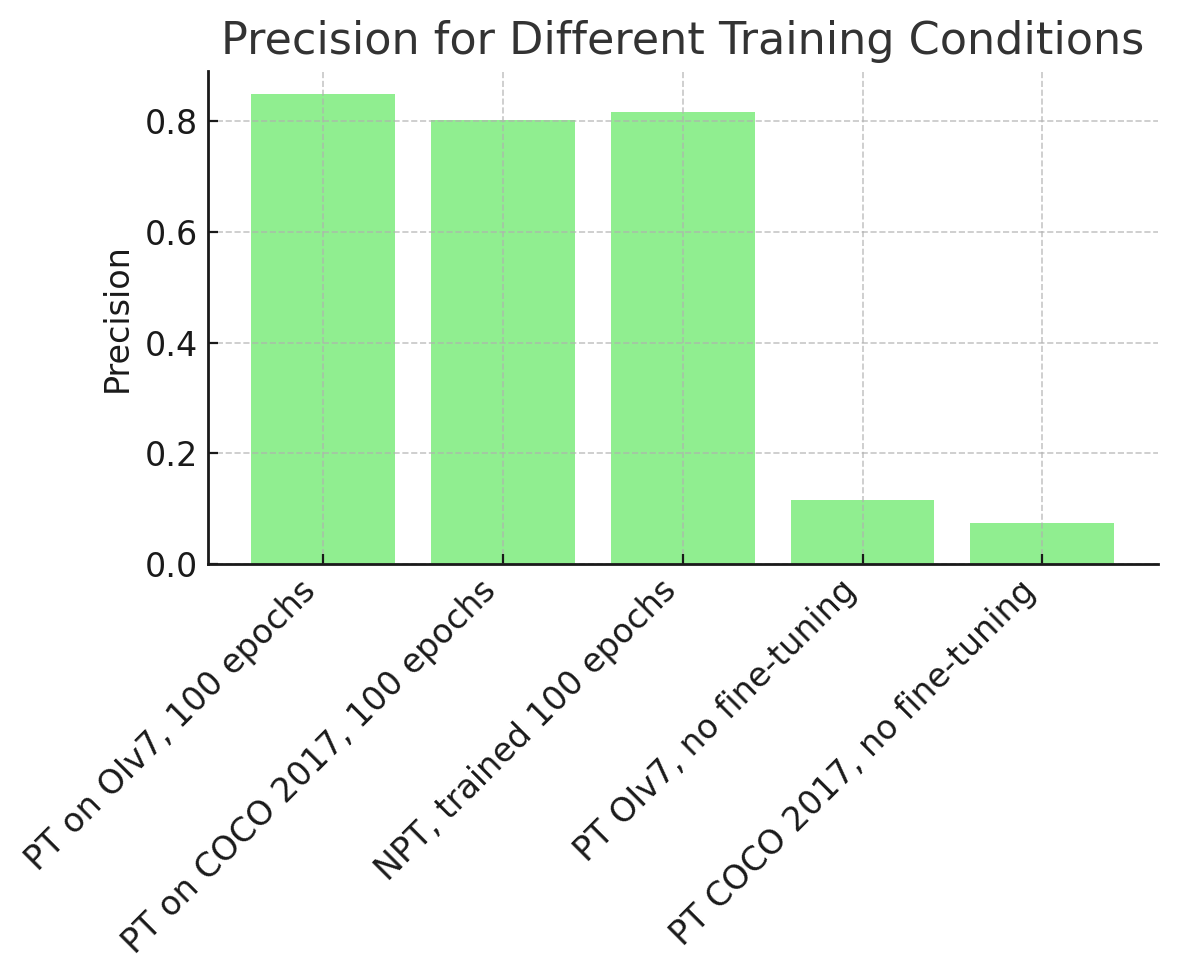
\includegraphics[width=0.8\linewidth]{precision.png}
    \caption{Precision across different training conditions}
    \label{fig:precision}
\end{figure}

\begin{figure}[H]
    \centering
    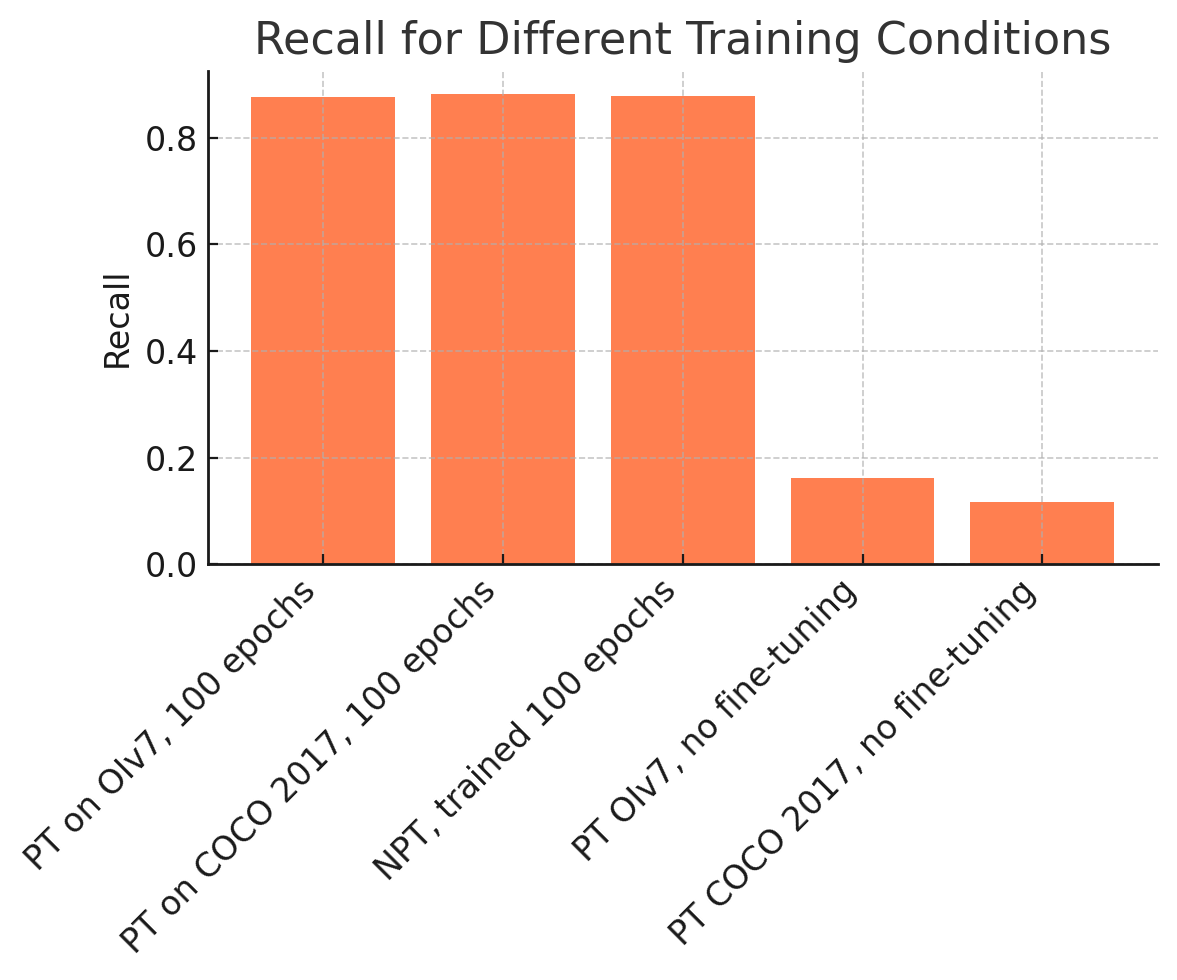
\includegraphics[width=0.8\linewidth]{recall.png}
    \caption{Recall across different training conditions}
    \label{fig:recall}
\end{figure}

\begin{figure}[H]
    \centering
    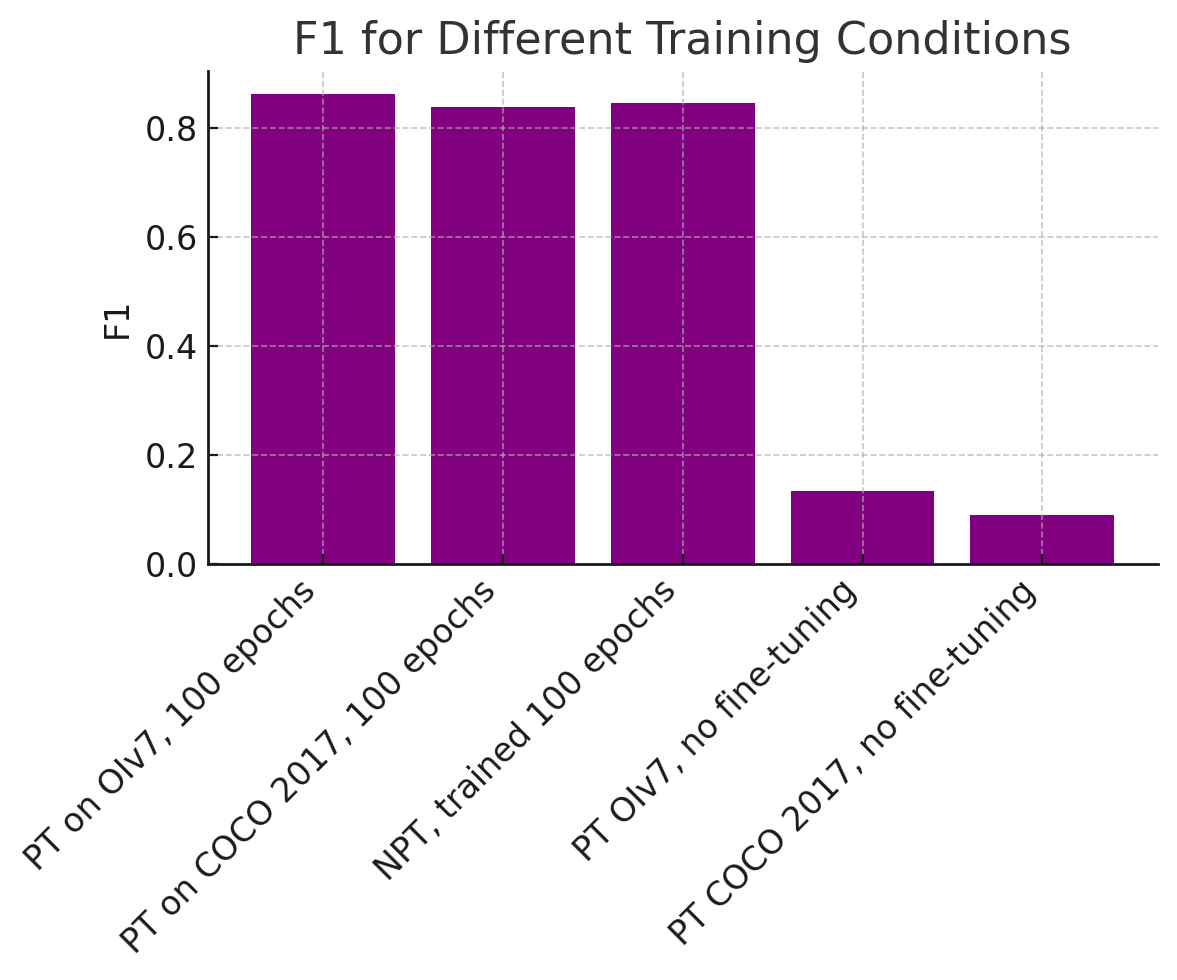
\includegraphics[width=0.8\linewidth]{f1.png}
    \caption{F1 Score across different training conditions}
    \label{fig:f1}
\end{figure}

As visible in Figures 3-6, all models trained or fine-tuned on the dataset performed significantly better than the pre-trained models without fine-tuning. The models show similar performance in regards to the above metrics, potentially showing that a larger version of YOLOv8 should have been chosen with more parameters to potentially differentiate between the various model types. Larger models have increased capacity for learning complex features, or may generalize better, at the risk of over fitting~\cite{model_complexity}. This would allow us to potentially notice a bigger performance difference between models, with potentially for even higher scoring on metrics such as the F1 Score. Ultimately, as visible in Appendix C Table 6, the fine-tuned model that was pre-trained on OpenImages v7 would be our choice for deployment in a robotics application. It had a high amount of true positives comparable to the other fine-tuned model or when training from scratch, while maintaining the lowest amount of false positives between different conditions. This may support our hypothesis of a 'cart' class in pre-training improving post fine-tuning performance. Additionally, this model had the highest IoU and F1 between our models despite only by a few percentage points, further supporting our decision.

\section{Robotic Integration: A Review}
The modern landscape of robotics offers unique opportunities and challenges. As technology progresses, the integration of computer vision and robotics in pragmatic applications becomes more feasible and valuable. We explore such integration in the context of retail environments, especially focusing on shopping cart management, and propose a framework to simplify this process.

While a popular concept among modern robotics research is self-driving shopping carts~\cite{self-driving}, realizing this idea requires a complete overhaul of the ongoing trolley system in retail environments, resulting in high financial costs.

Instead, we propose a framework with a surveillance system that adopts YOLOv8 to perform bounding box detection on shopping carts in-store and in the vicinity. A stationary agent would then determine if the cart is unattended; if yes, it would signal an agent equipped with robotic arms to retrieve the cart. Conversely, a single, stationary agent with a mounted camera system could execute all the tasks above.

\subsection{Unattended Object Recognition}
Identifying whether a shopping cart has been unattended is crucial: the system should restrain from snatching away a cart currently in use. The feasibility of unattended object recognition was demonstrated by Jadhav and Momin~\cite{detection-identifcation} using the following methods (the points are directly quoted):
\begin{itemize}
    \item{\textbf{Foreground Blob Extraction:}}
    Key features such as the location, height, and width of each blob are extracted, critical for subsequent object identification tasks.
    \item{\textbf{Object Classification:}}
    Objects are classified into three categories: stationary, removed, and moving, based on the lengths of their foregrounds.
\begin{table}[h]
\centering
\begin{tabular}{lcc}
\toprule
\textbf{Long Foreground} & \textbf{Short Foreground} & \textbf{Object Type} \\
\midrule
1 & 0 & Stationary Object \\
0 & 1 & Removed Object \\
1 & 1 & Moving Object \\
\bottomrule
\end{tabular}
\caption{Object Classification with Two Foregrounds~\cite{detection-identifcation}}
\label{tab:object_classification}
\end{table}
\item{\textbf{Object Identification and Responsive Actions:}}
If a static object is recognized as a person, it remains classified as such. If ambiguity exists, such as a person appearing stationary for long periods, the decision is deferred for manual review. Conversely, if an object is left unattended, the system takes note of this instance. This approach to object classification complements our focus on refining object recognition processes in environments like shopping centers.
\end{itemize}

While the specific techniques may need to be adjusted in the context of unattended cart identification, Jadhav and Momin's methodology~\cite{detection-identifcation} serves as a foundational building block for our task.

\subsection{Navigation}
Mobile navigation poses another foundational challenge. As robots are deployed in retail settings, they must not only navigate through fixed structures but also adapt to transient changes such as moving people, temporary displays, and varying crowd densities. Our exploration of the agent's navigation is two-fold, both in terms of global and local navigation.

\subsubsection{Global Navigation}
In global navigation, the agent has access to prior knowledge of the environment~\cite{mobile-robot-navigation}. Global navigation refers to the robot's ability to orient itself and plan routes within the larger environment. The most prominent methods developed for global navigation are the Voronoi Graph, Dijkstra Algorithm, and Visibility Graph ~\cite{mobile-robot-navigation}.

\subsubsection{Local Navigation}
In local navigation, the robot can control its movement and direction autonomously with equipped sensors like ultrasonic, infrared, and camera sensors~\cite{mobile-robot-navigation}. Common algorithms to solve the local navigation problem are Fuzzy Logic, Neural Network, Genetic Algorithm, and Simulated Annealing~\cite{mobile-robot-navigation}.

Fuzzy logic plays a critical role in enhancing the capabilities of local navigation systems in complex and dynamic environments such as retail settings~\cite{intro-fuzzy}. Unlike traditional binary logic systems that represent truth values in 0-1, fuzzy logic introduces a spectrum of possibilities and enables robots to make decisions in ambiguous scenarios with hidden information~\cite{intro-fuzzy}.

\subsection{Robotic Arm Grip}
With the unattended object identified and navigation enabled, the mobile agent is ready to retrieve the shopping cart. A core component in object retrieval is determining the gripping method of the agent's arm, which involves the type of grip system, the gripping strength, and the adaptability to various shapes and sizes of the object to be retrieved.
Determining an appropriate gripper design is crucial for ensuring efficient object retrieval by the mobile agent. Typically, the design type is a product of the following parameters: size, shape, and material~\cite{robotic-arm}. We determine the following parameters for the handle of a general shopping cart:

\begin{table}[h]
\centering
\begin{tabular}{lc}
\hline
\textbf{Size} & 31.5 mm to 80 mm\\
\hline
\textbf{Shape} & Circular\\
\hline
\textbf{Material} & Rocks / Electronics \\
\hline
\textbf{Type} & Daily Objects \\
\hline
\end{tabular}
\caption{Shopping Cart Handle Parameters}
\label{Shopping Cart Handle Parameters}
\end{table}

Given these conditions, the most fitting category of gripper system for a shopping cart is Completely constrained-rigid link, with Under-constrained-rigid link as a close second~\cite{robotic-arm}. Recommended structures of the gripper system for these two categories are linear actuator, rotary actuator, pneumatic actuator, cable-driven, and electromagnet~\cite{robotic-arm}.

\section{Framework}
We propose the following framework/pipeline (Figure \ref{framework}) that integrates the fine-tuned YOLOv8 model, unattended object recognition, navigation, and robotic arm cart retrieval.

\begin{figure}[ht]
    \centering
    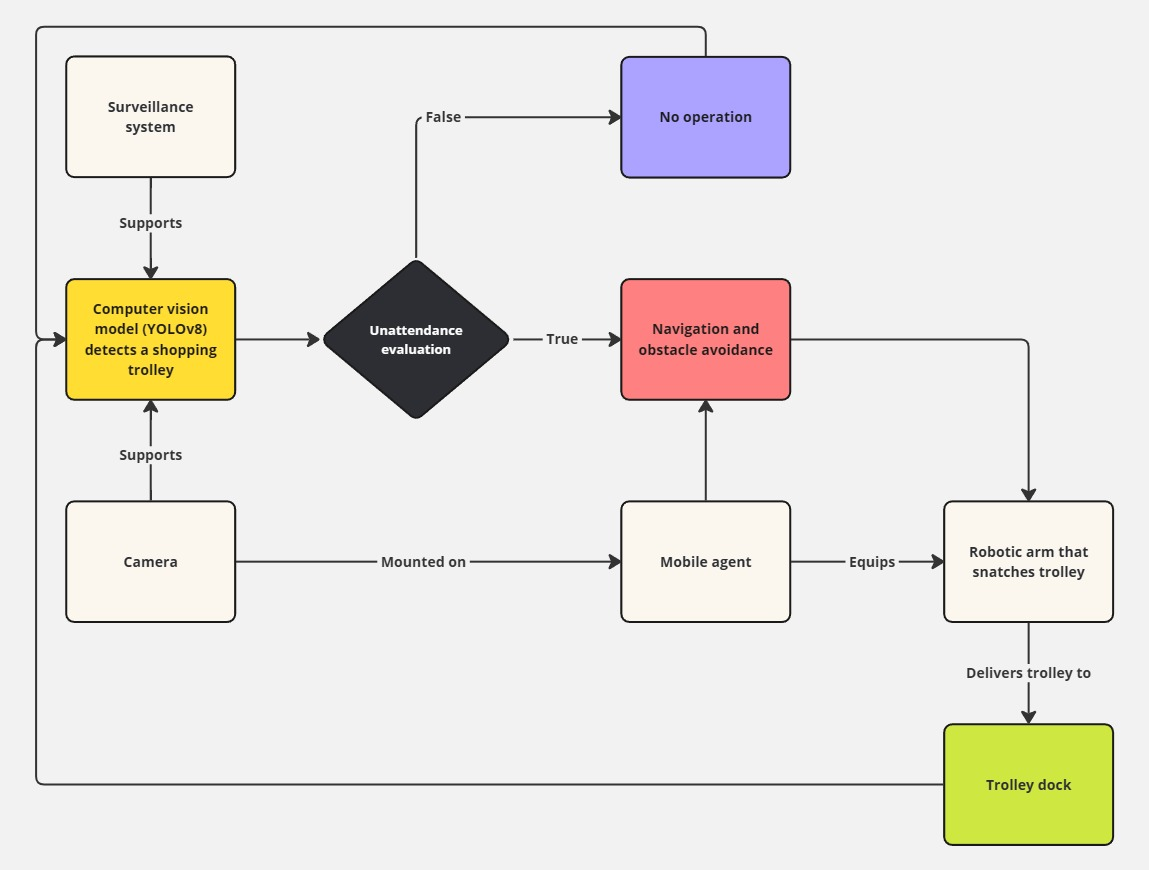
\includegraphics[width=0.5\textwidth]{images/Pipeline.jpg}
    \caption{A Comprehensive Framework}
    \label{framework}
\end{figure}

This framework describes a system that utilizes a computer vision model (YOLOv8) to detect unattended shopping trolleys in a retail environment. 
\begin{enumerate}
  \item \textbf{Surveillance System:} A camera feeds live images to the system.
  \item \textbf{Computer Vision Detection:} These images are processed by the YOLOv8 model to detect shopping trolleys.
  \item \textbf{Unattendance Evaluation:} If a trolley is detected as unattended, the system activates further operations. If not, no action is taken.
  \item \textbf{Navigation and Obstacle Avoidance:} Once an unattended trolley is confirmed, a mobile agent (likely a robot) equipped with navigation and obstacle avoidance capabilities is activated.
  \item \textbf{Trolley Retrieval:} The mobile agent uses a robotic arm to physically retrieve the trolley.
  \item \textbf{Trolley Docking:} Finally, the mobile agent delivers the trolley to a designated dock.
\end{enumerate}

This automated process aims to efficiently manage shopping trolley retrieval, reducing labor and improving store operations.

\section{Conclusion}
We have developed and validated a comprehensive framework that employs the advanced capabilities of the YOLOv8 model for the automated retrieval of shopping carts in retail environments. 

Our experimental results, derived from training and testing the robust dataset by Kornilov~\cite{kornilov-dataset}, demonstrate that the fine-tuned YOLOv8 (especially with un-pretrained weights) performs exceptionally well in detecting shopping carts under diverse conditions, achieving high values in IoU, precision, recall, and F1 metrics. This underscores the effectiveness of leveraging deep neural networks for real-world applications.

Moreover, the proposed robotic integration framework, which includes components for unattended object registration, sophisticated navigation systems, and a robust gripping mechanism, paves the way for practical deployment in commercial environments. This system reduces the dependence on human labor by automating manual tasks.

Future work will focus on refining the detection algorithms to handle more complex scenarios, such as varying light conditions and crowded scenes. Additionally, exploring the integration of artificial intelligence (AI)-driven decision-making processes can further enhance the system's autonomy and efficiency.

In conclusion, this study not only contributes to the fields of computer vision and robotics but also presents a viable solution to a common logistical problem faced by retailers globally, demonstrating the transformative potential of AI in industry.


\section*{Acknowledgements}
Our heartfelt thanks go out to Dr. Chenliang Xu, Susan Liang, Luchuan Song, and Pinxin Liu for their guidance on this paper. Susan Liang suggested we look into the challenging yet meaningful frontiers of robotics, which significantly spearheaded the direction of our research.

{\small
\bibliographystyle{ieeenat_fullname}
\bibliography{main}}

\appendix

\section{Appendix A}

This appendix includes an illustration of our model's bounding box detection, where green boxes are the predictions and red boxes are the ground truth.

\begin{figure}[H]
    \centering
    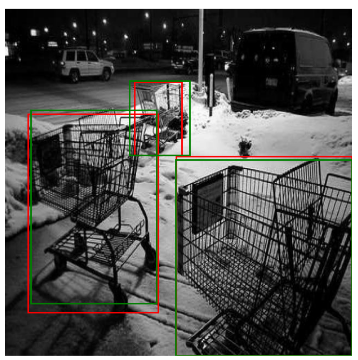
\includegraphics[width=0.8\linewidth]{images/bounding-box-detection.png}
    \caption{Bounding Box Detection}
    \label{fig:bb}
\end{figure}

\section{Appendix B}
This appendix includes confusion matrices of all our pretrained and non-pretrained models, with and without dataset training~\cite{kornilov-dataset}, based on true positives, false positives, and false negatives.

\begin{figure}[H]
    \centering
    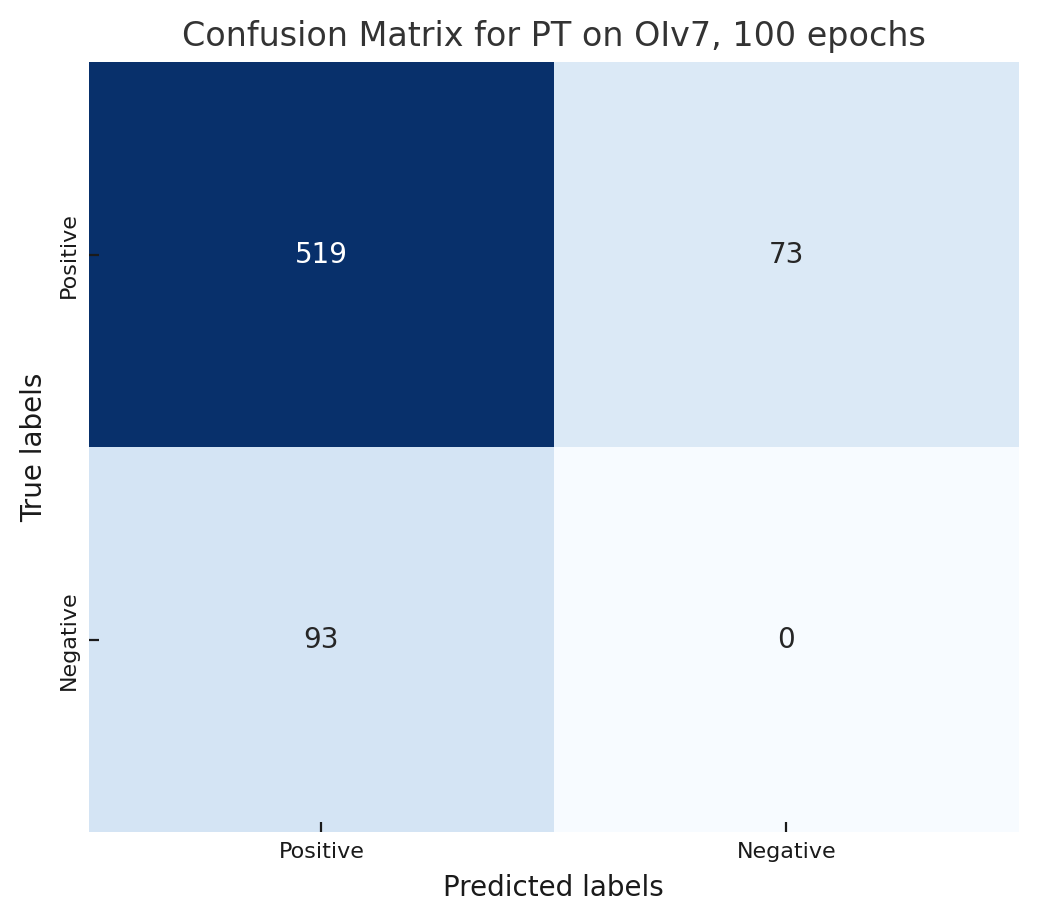
\includegraphics[width=0.8\linewidth]{cmptoiv7100.png}
    \caption{PT on OIv7, 100 epochs}
    \label{fig:cmptoiv7100}
\end{figure}

\begin{figure}[H]
    \centering
    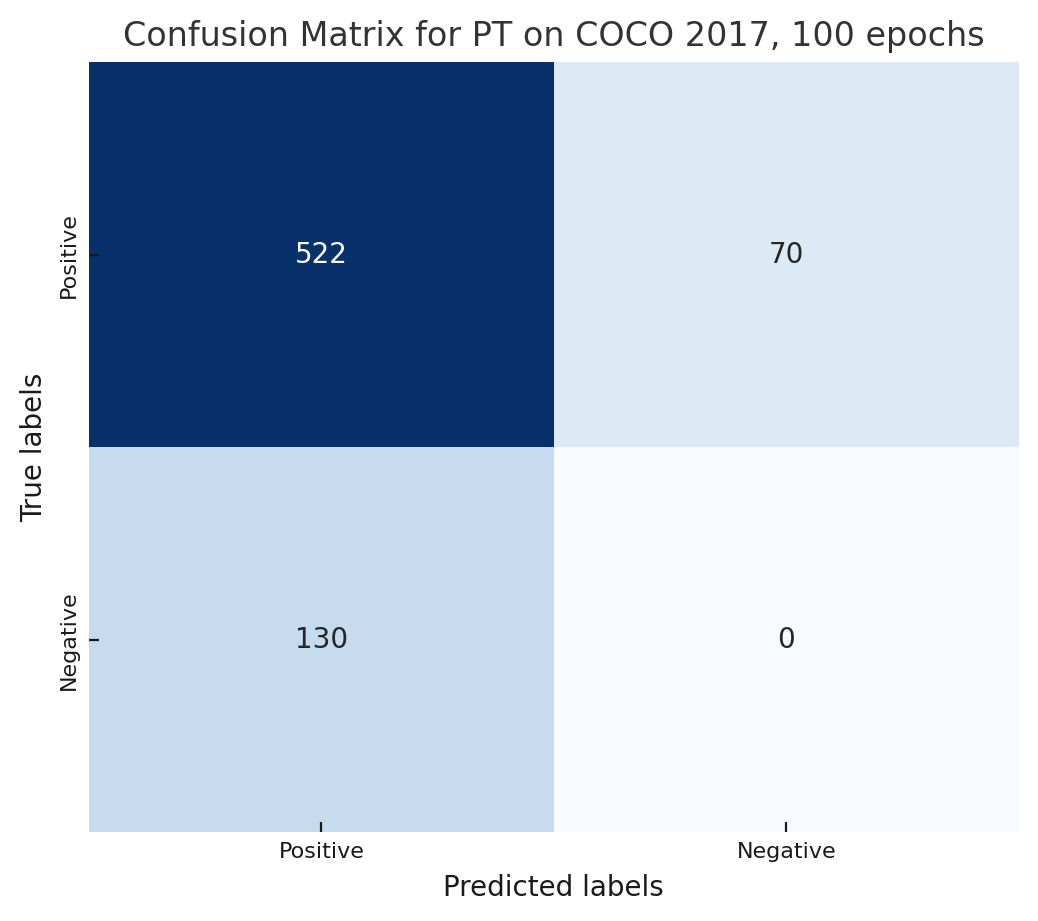
\includegraphics[width=0.8\linewidth]{cmptcoco100.png}
    \caption{PT on COCO 2017, 100 epochs}
    \label{fig:cmptcoco100}
\end{figure}

\begin{figure}[H]
    \centering
    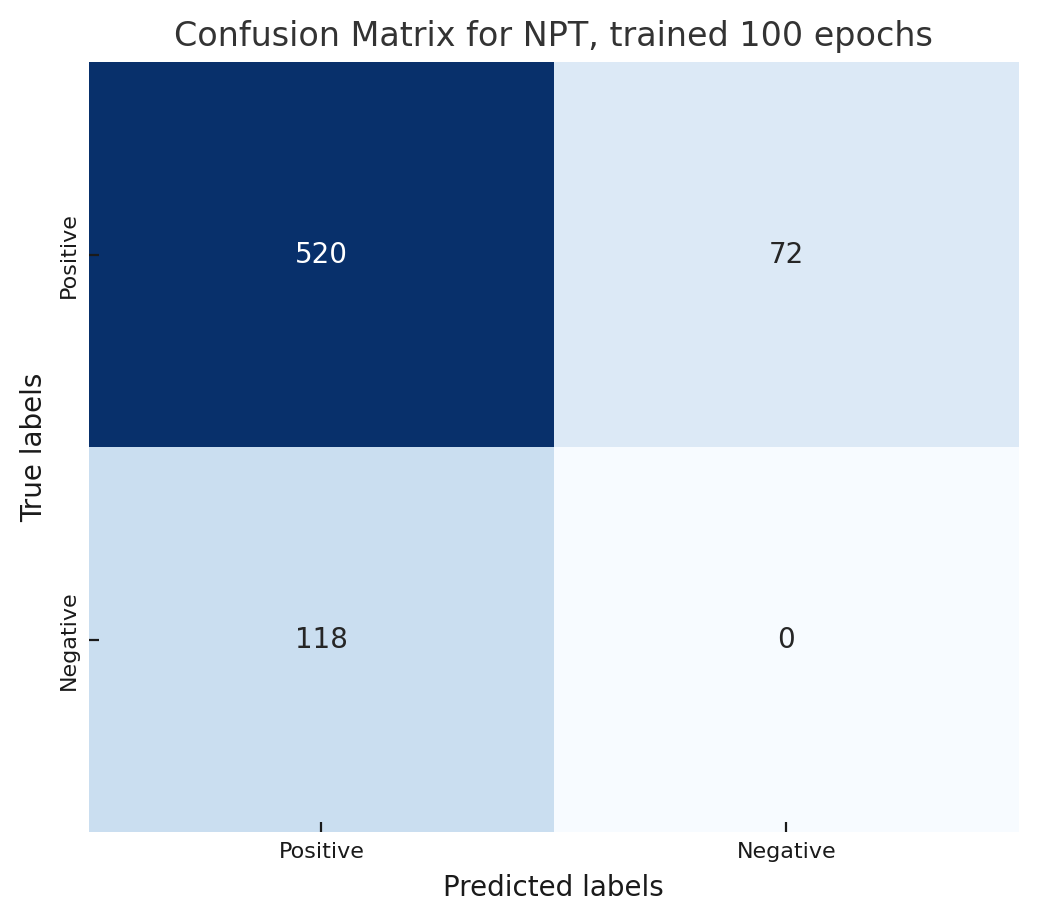
\includegraphics[width=0.8\linewidth]{cmnpt100.png}
    \caption{NPT, trained 100 epochs}
    \label{fig:cmnpt100}
\end{figure}

\begin{figure}[H]
    \centering
    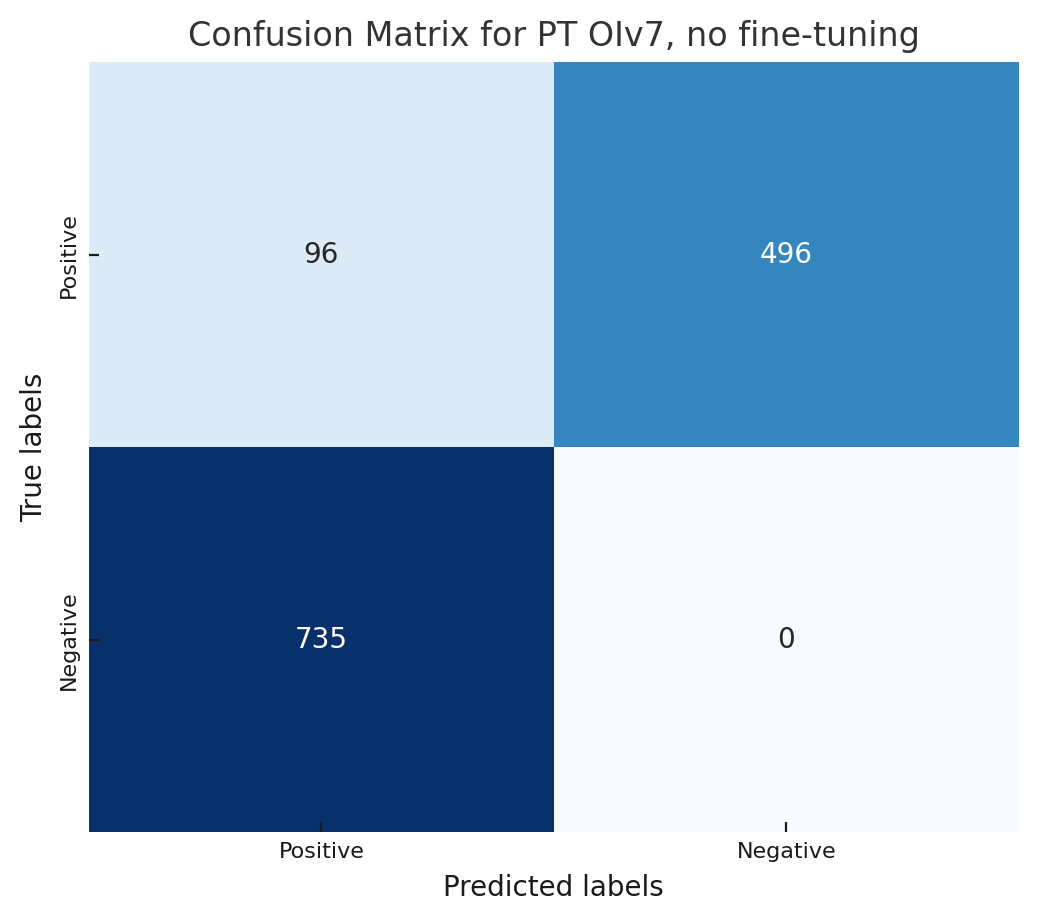
\includegraphics[width=0.8\linewidth]{cmptoiv7nft.png}
    \caption{PT OIv7, no fine-tuning}
    \label{fig:cmptoiv7nft}
\end{figure}

\begin{figure}[H]
    \centering
    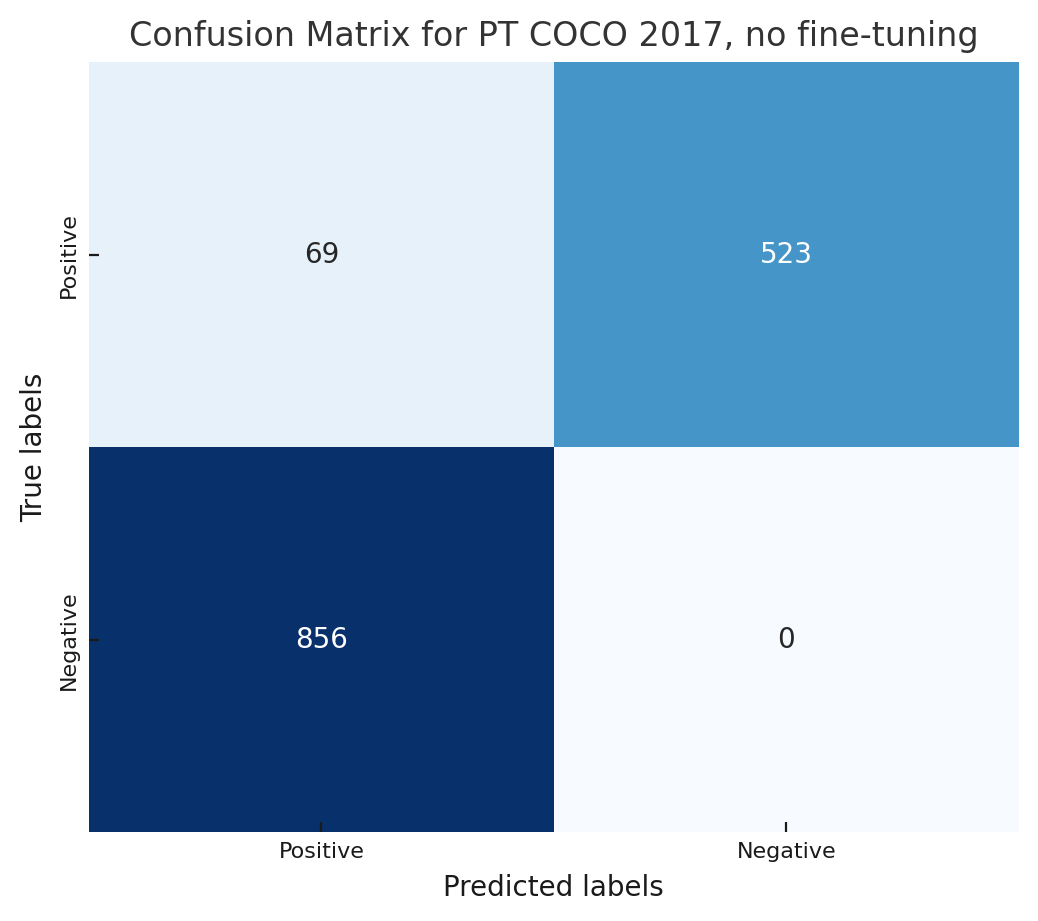
\includegraphics[width=0.8\linewidth]{cmptcoconft.png}
    \caption{PT COCO 2017, no fine-tuning}
    \label{fig:cmptcoconft}
\end{figure}

\onecolumn

\section{Appendix C}
This appendix includes raw values supporting the metrics graphs above and confusion matrices in appendix A.

\begin{table}[H]
\centering
\caption{YOLOv8n: Performance Scores under Various Training Conditions}
\label{tab:performance_scores}
\begin{tabular}{|l|c|c|c|c|}
\hline
\textbf{Model} & \textbf{Average IoU} & \textbf{Precision} & \textbf{Recall} & \textbf{F1} \\ \hline
Pretrained on OIv7, 100 epochs & 0.8671 & 0.8480 & 0.8767 & 0.8621 \\ \hline
Pretrained on COCO 2017, 100 epochs & 0.8739 & 0.8006 & 0.8818 & 0.8392 \\ \hline
Pretrained OIv7, no fine-tuning & 0.2268 & 0.1155 & 0.1622 & 0.1349 \\ \hline
Pretrained COCO 2017, no fine-tuning & 0.1725 & 0.0746 & 0.1166 & 0.0909 \\ \hline
Non-pretrained, trained 100 epochs & 0.8693 & 0.815 & 0.8784 & 0.8455 \\ \hline
\end{tabular}
\end{table}

\begin{table}[H]
\centering
\caption{YOLOv8n: Detection Counts under Various Training Conditions}
\label{tab:detection_counts}
\begin{tabular}{|l|c|c|c|}
\hline
\textbf{Model} & \textbf{True Positives} & \textbf{False Positives} & \textbf{False Negatives} \\ \hline
Pretrained on OIv7, 100 epochs & 519 & 93 & 73 \\ \hline
Pretrained on COCO 2017, 100 epochs & 522 & 130 & 70 \\ \hline
Pretrained OIv7, no fine-tuning & 96 & 735 & 496 \\ \hline
Pretrained COCO 2017, no fine-tuning & 69 & 856 & 523 \\ \hline
Non-pretrained, trained 100 epochs & 520 & 118 & 72 \\ \hline
\end{tabular}
\end{table}


\end{document}